\documentclass[10pt]{article}
\usepackage{geometry}
\geometry{top=20mm, bottom=20mm, left=20mm, right=20mm}

\usepackage[english]{babel} 
\usepackage[utf8]{inputenc}
\usepackage[T1]{fontenc}
\usepackage{lmodern}

\usepackage{booktabs} 
\usepackage{amsmath}
\usepackage{amssymb}
\usepackage{amsfonts}
\usepackage{xspace}

\usepackage{url}
\usepackage[mode=buildnew]{standalone}
\usepackage{microtype}
%\usepackage[binary-units]{siunitx}
\usepackage{xcolor}
\usepackage{listings}
\lstloadlanguages{C++}
\lstset{
    language=C++,
    numbers=left,
    numberstyle=\footnotesize,
    numbersep=5pt,
    showspaces=false,
    showstringspaces=false,
    showtabs=false,
    tabsize=1,
    captionpos=b,
    breaklines=true,
    breakatwhitespace=false,
    escapeinside={(*@}{@*)},
    morekeywords={andnot, function, var, to, step, cmpgt, cmplt, if,
        then, else, endif, wenn, solange, wahr, falsch, sonst},
    basicstyle=\ttfamily,
    commentstyle=\itshape\color{blue},
%    keywordstyle=\bfseries\color{darkblue},
    stringstyle=\color{darkred},
    literate={:=}{{$\gets$}}1 {<=}{{$\leq$}}1 {>=}{{$\geq$}}1
    {!=}{{$\neq$}}1 {*}{{$\cdot$}}1,
    mathescape=true,
    texcl=true
    %xleftmargin=1cm
}

%\usepackage{tikz}
%\usetikzlibrary{shapes.geometric,arrows,calc,decorations.pathreplacing}
\usepackage{placeins}
\usepackage{enumitem}
%\setlist[description]{style=multiline,leftmargin=3cm}

\usepackage{subcaption}


\title{GSPC19 Architecture}
%\shorttitle{GSPC Architecture} % gets used in the footer
%\subtitle{Proposal}

% comma separated list of authors
%\author{Author}
\date{}


\newcommand{\user}{User\xspace}
\newcommand{\rts}{RTS\xspace}
\newcommand{\sched}{Scheduler\xspace}
\newcommand{\worker}{Worker\xspace}
\newcommand{\workers}{Workers\xspace}
\newcommand{\rman}{RM\xspace} 
\newcommand{\iml}{IML\xspace}
\newcommand{\we}{WE\xspace}
\newcommand{\rif}{RIF\xspace}

\newcommand{\rdag}{DAG\xspace}
\newcommand{\rdagrep}{DAG\_report\xspace}
\newcommand{\js}{JobServ\xspace}
\newcommand{\task}{Task\xspace}
\newcommand{\res}{Res\xspace}
\newcommand{\rc}{RClass\xspace}
\newcommand{\pref}{Preference\xspace}
\newcommand{\req}{Requirement\xspace}

\newcommand{\id}{::ID\xspace}
\newcommand{\conn}{::Connection\xspace}

\begin{document}

\maketitle
%\tableofcontents
%\newpage

% set up page
%\RaggedRight

\section{Introduction}
This document describes the new architecture for GSPC19, focusing on scheduling
and on the interaction between components.


\section{Architecture}
The main components shown in Figure~\ref{fig:architecture} are described as follows, together with a set of definitions that will be used in this document.
\begin{figure}[t]
    \centering
    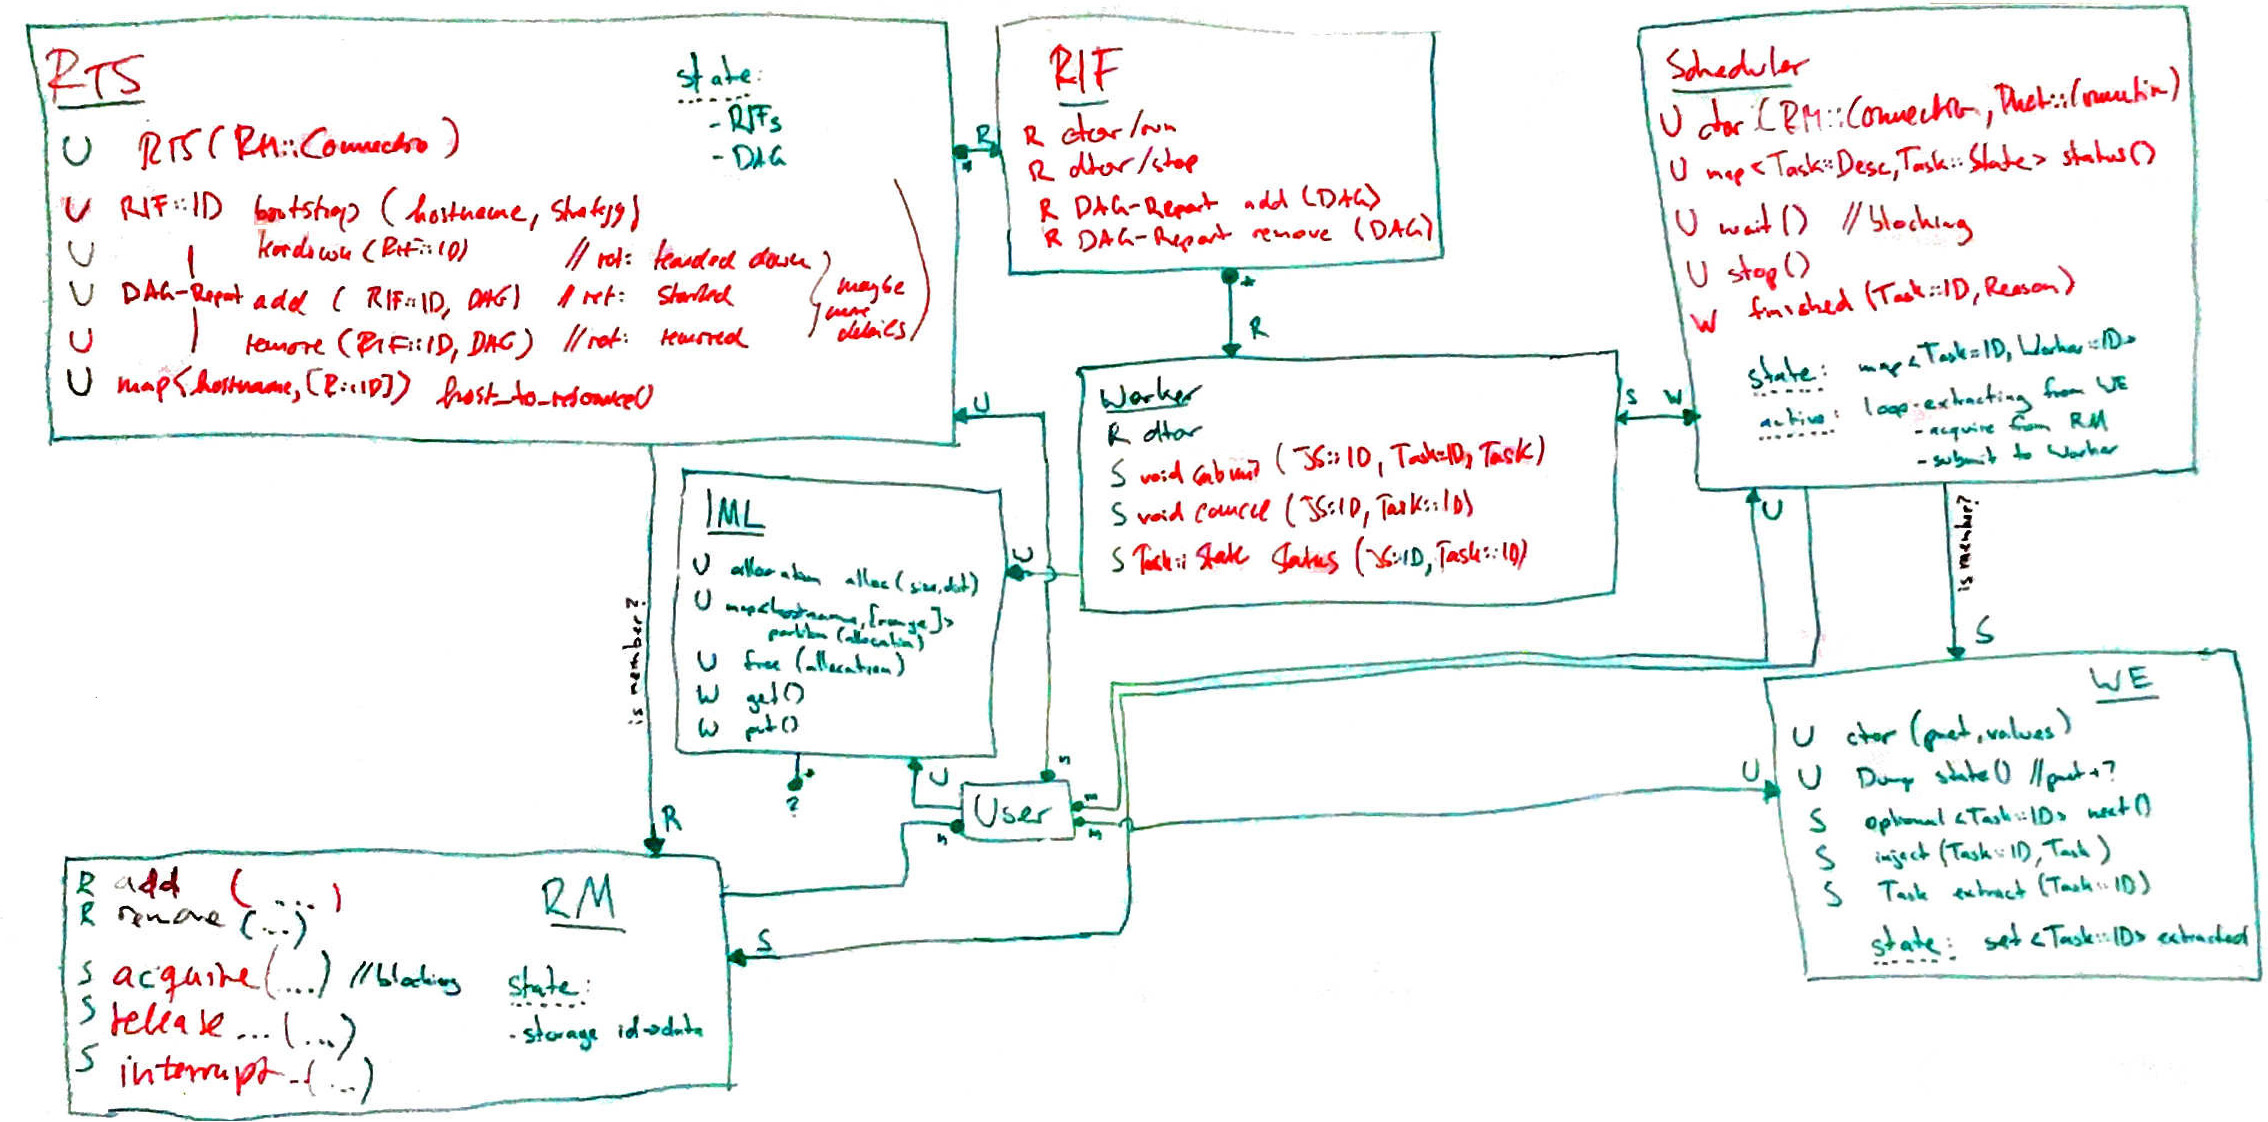
\includegraphics[width=.9\linewidth]{./api_overview.jpg}
    \caption{GSPC19 Architecture}
    \label{fig:architecture}
\end{figure}
%
\begin{table}[ht]
    \centering
    \caption{Terms used in this document}
    \label{tab:terms}
    \bgroup
    \setlength{\tabcolsep}{2em}
    \begin{tabular}{ll}
        \toprule
        \res & Resource; each resource in the system \\ 
                        & is associated with a unique ID \\
        \rc & Resource class; type of resources (e.g., core, socket, node, GPU)\\
        \task & GPISpace activity; includes an ID, state, description (e.g., ports, modules), \\
                        & associated resource class \\
        \rdag & DAG of Resources (hierarchical representation of resources, describing \\
                        & the dependencies between existing resource IDs, based on their \\
                        & class; e.g., a socket includes multiple cores) \\
        \rdagrep &  DAG Report; connection information for each resource in a given DAG \\
        \pref & Resource preference; represents a list of specific resource IDs, \\
                        & one of which should be  allocated by the scheduler for a given task \\
        \req  & Requirement; represents a list of tuples (resource class, list of preferences) \\   
                        & to be used for co-allocation scheduling: the task requires one resource for \\
                        & each element of the list, defined by the given class and preferences  \\ 
        \midrule
        \js & Job Server \\
        \rts & Run-Time System \\
        \iml & Independent Memory Layer \\
        \bottomrule
    \end{tabular}
    \egroup
\end{table}
%

\subsection{RTS -- The Run-Time System}
The \emph{Run-Time System} is in charge of initializing RIF daemons on each
compute node, as well as starting (or connecting to an existing) Resource
Manager.
The \emph{Run-Time System} also keeps track of all the resources associated with
its physical machines and of the mapping between resources, hostnames, and
corresponding RIF processes.

It interacts with the following components:
\begin{description}
    \item [\rif:] The \rts can start/stop multiple \rif daemons
    \item [\rman:] The \rts works in conjunction with one \rman; whereas the
    \rts manages the connections to physical resources, the \rman keeps track of
    usage and allocations for the same set of resources  
    \item [\user:] The user is the only component in charge (and capable) of
    initializing and configuring the \rts
\end{description}
%
\begin{table}[ht]
    \centering
    \caption{Run-Time System}
    \label{tab:rts}
    \bgroup
    \setlength{\tabcolsep}{2em}
    \begin{tabular}{ll}
        \toprule
        Caller & Method \\
        \midrule
        \user & \rts(\rman\conn) \\
        \user & \rif\id bootstrap(hostname, strategy) \\
        \user & \rif\id teardown(\rif\id)    // ret: toredown \\
        \user & \rdagrep add(\rif\id, \rdag) // ret: started \\
        \user & \rdagrep remove(\rif\id, \rdag) // ret: removed \\
        \user & map<hostname, [\res\id]> host\_to\_resource() \\
        \midrule
        & Data members \\        
        \midrule
        & RIFs \\
        & DAGs \\
        \bottomrule
    \end{tabular}
    \egroup
\end{table}
%

\subsection{RIF}

The \rif daemon is a process that runs on each compute node managed by GPISpace
and manages the GPISpace resources defined for that particular machine.
Each resource ID is associated with a worker that can execute tasks defined for
that type of resource.
Upon receiving a resource description (DAG describing the resource hierarchy for
the node), the \rif daemon is in charge of starting a worker for each resource
in the DAG, and return the connection information for each worker back to the
user.
The \rif should provide transparent access to workers to the \rts, that is it
should make connection information available for each resource it manages. The
\rif could then act as a proxy and forward tasks to the right worker or allow
external processes to connect to workers directly.

It interacts with the following components:
\begin{description}
    \item [\worker:] The \rif can start/stop multiple \workers (either as
    processes or as threads); it can potentially handle pinning to cores for
    specific workers (e.g., socket workers)
    \item [\rts:] The \rts manages all the communication with all the \rif
    daemons in the system, and forwards the worker information to the user
    \item [\iml:] Currently, the \rif initializes the \iml on the node it is 
    responsible for
\end{description}
%
\begin{table}[ht]
    \centering
    \caption{RIF}
    \label{tab:rif}
    \bgroup
    \setlength{\tabcolsep}{2em}
    \begin{tabular}{ll}
        \toprule
        Caller & Method \\
        \midrule
        \rts & ctor/run \\
        \rts & dtor/stop \\
        \rts & \rdagrep add(\rdag)  \\
        \rts & \rdagrep remove(\rdag) \\
        \midrule
        \rts & start\_iml() // current implementation \\
        \bottomrule
    \end{tabular}
    \egroup
\end{table}
%

\subsection{Worker}
The \worker is the component that executes workflow tasks on compute nodes. A
\worker is a process/thread associated with a specific resource ID and can only
execute tasks requiring that type of resource.

Instead of executing a single task at a given moment, a worker may be
implemented to overlap communication (incoming data transfers, outgoing data
transfers) with the computation phase of another task.
Thus it needs to keep track of the three tasks that may run concurrently, and to
synchronize their phases.
Furthermore, the failure of one of these running tasks should  trigger the
failure/cancellation of the others.

\workers interact with the following components:
\begin{description}
    \item [\sched:] The \sched starts/cancels tasks on any worker, and can as
    well interrogate the status of a given task
    \item [\rts:] The \rts manages the creation of workers and keeps track of
    connection information for each \worker
    \item [\iml:] The \worker needs access to the global memory in order to
    perform memory transfers
\end{description}

%
\begin{table}[ht]
    \centering
    \caption{Worker}
    \label{tab:worker}
    \bgroup
    \setlength{\tabcolsep}{2em}
    \begin{tabular}{ll}
        \toprule
        Caller & Method \\
        \midrule
        \rts & ctor \\
        \rts & dtor \\
        \sched & void submit(\js\id, \task\id, \task)  \\
        \sched & void cancel(\js\id, \task\id) \\
        \sched & \task::State status(\js\id, \task\id) \\
        \bottomrule
    \end{tabular}
    \egroup
\end{table}
%


\subsection{RM -- Resource Manager}

The Resource Manager is the component that keeps track of all existing resources in the system, together with their state (available or in use). 

Interactions:
\begin{description}
    \item [\sched:] The scheduler is the only component that can acquire/release resources (but the system should allow for multiple schedulers to use the same \rman, for instance to have multiple applications running on the same physical machines). The \rm provides a means to mark resources that are in use, while taking into account resource hierarchies; this is done in a transparent manner relative to the scheduler, which only needs to keep track of the class of resource it needs, without any knowledge of dependent resources
    \item [\rts:] The \rts can add and remove resource hierarchies (DAGs) from the \rm
\end{description}

In the case of scheduling with preferences, we define the following types:
\begin{itemize}
    \item \pref := [\res\id]
    \item \req := (\rc, [\pref])
\end{itemize}

%
\begin{table}[ht]
    \centering
    \caption{Resource Manager}
    \label{tab:rm}
    \bgroup
    \setlength{\tabcolsep}{2em}
    \begin{tabular}{ll}
        \toprule
        Caller & Method \\
        \midrule
        \rts & add(\rdag<\res\id>) \\
        \rts & remove(\rdag<\res\id>) \\
        \sched & acquire(\js\id, \rc) // blocking, return \res\id  \\
        \sched & release(\js\id, \res\id) \\ 
        \sched & release(\js\id, [\res\id]) \\
        \sched & interrupt(\js\id) \\
        \midrule
        \sched & acquire(\js\id, [\rc]) // blocking, co-allocation, 
        return [\res\id]  \\
        \sched & acquire(\js\id, [\req]) // blocking, 
        scheduling with preferences, return [\res\id]  \\
        \sched & acquire(\js\id, \rc, [memsize]) // blocking, 
        return (\res\id,[Mem\id, offset])  \\
        \midrule
        & Data members \\
        \midrule
        & Storage id -> data \\
        \bottomrule
    \end{tabular}
    \egroup
\end{table}
%

Possible issues with the acquire/release blocking interface of the Resource
Manager:
\begin{description}
    \item [Deadlock] Can occur when acquiring a set of resources in a single
    call 
    \item [Livelock] Similar to the deadlock situation, in the case of requiring
    multiple resources within the same blocking acquire
    \item [Class conflict] Starvation may occur in the following cases
    Resources from different classes are required by concurrent
    \emph{acquire} calls, e.g., nodes and cores are requested in the same time.
    Fulfilling the request for \emph{cores} may result in never having a \emph{node}
    available and thus starving the \emph{node}-level requests.
    
    Another resource class issue might be due to the blocking nature of the
    \emph{acquire} call. 
    Example:
    An application with two types of tasks, IO and computational (Calc)
    tasks that run on separate classes of resources. Let us assume the workflow
    engine generates many IO tasks followed by corresponding Calc tasks, each of
    which can be executed as soon as one IO task is finished.
    However, since the number of available IO workers is limited, the
    scheduler may block in an IO \emph{acquire} call and only start processing the
    Calc tasks when all the IO tasks are done.
    Such behavior may be avoided by implementing class-aware task
    generation at the workflow engine level or class-aware scheduling.
    
\end{description}


\subsection{Scheduler}
The \sched is the component that provides flexibility to GPISpace, in particular
by allowing for the implementation of multiple scheduling policies to match
application needs.
A possible basic implementation is described in the following section, along
with several policies targeted at specific use cases. 

Interactions:
\begin{description}
    \item [\user:] The scheduler is started upon its creation by the user; it
    provides the user with a method to wait for the end of the workflow execution,
    as well as a stop function to cancel running tasks 
    \item [\worker:] The \worker executing a task has to be able to notify the
    \sched that the execution has finished, either successfully or due to a
    failure/cancel.
\end{description}
%
\begin{table}[ht]
    \centering
    \caption{Scheduler}
    \label{tab:sched}
    \bgroup
    \setlength{\tabcolsep}{2em}
    \begin{tabular}{ll}
        \toprule
        Caller & Method \\
        \midrule
        \user & ctor(\rman\conn, Pnet\conn) \\
        \user & map<\task::Desc, \task::State> status() \\
        \user & wait() // blocking  \\
        \user & stop() \\
        \worker & finished(\task\id, Reason) \\
        \midrule
        & Data members \\
        \midrule
        & map<\task\id, \worker\id> \\
        \bottomrule
    \end{tabular}
    \egroup
\end{table}
%


\subsection{WE -- Workflow Engine}
\label{sec:we}
The workflow engine is a simplified version of the current workflow engine of
GPISpace, which only needs to be able to handle one workflow (specified by the
user at the \we creation) instead of an arbitrary number of concurrent
workflows. 
Its role is to extract available tasks and inject results back into the
workflow. It also has to provide a method that informs the user of the state of
the workflow, regardless of whether its execution has finished or not.

The most significant change with respect to the current implementation is that
the \we does not need to support a \emph{cancel} operation, as stopping the
workflow execution can simply be seen as ceasing the calls to  \emph{extract} at
the scheduler level. 

Interactions:
\begin{description}
    \item [\sched:] The scheduler drives the extraction of available tasks; it
    is also responsible for injecting the results of finished tasks back into the
    workflow
    \item [\user:] The \user initializes the \we based on the application
    workflow; it can at any moment discover the state of the workflow by directly
    interrogating the \we (regardless of whether the scheduler has finished the
    execution of the workflow)
\end{description}
%
\begin{table}[ht]
    \centering
    \caption{Workflow Engine}
    \label{tab:we}
    \bgroup
    \setlength{\tabcolsep}{2em}
    \begin{tabular}{ll}
        \toprule
        Caller & Method \\
        \midrule
        \user & ctor(pnet, values) \\
        \user & dump state() \\
        \sched & optional<\task\id> next()  \\
        \sched & inject(\task\id, \task) \\
        \sched & \task extract(\task\id) \\
        \midrule
        & Data members \\
        \midrule
        & set<\task\id> extracted \\
        \bottomrule
    \end{tabular}
    \egroup
\end{table}
%

\subsection{IML -- Independent Memory Layer}
The \iml handles the distributed global memory that spans over multiple 
physical machines.
Currently, the memory layer is not completely independent, as its 
initialization is handled by the \rif daemons. 

Interactions:
\begin{description}
    \item [\user:] The user is in charge of allocating memory ranges in the
    \iml; it can also require information about data partitioning, that is the
    mapping between allocated memory and physical machine hostnames where the 
    data is actually located
    \item [\worker:] Workers need access to the \iml to trigger
    incoming/outgoing data transfers
\end{description}
%
\begin{table}[ht]
    \centering
    \caption{Independent Memory Layer (IML)}
    \label{tab:iml}
    \bgroup
    \setlength{\tabcolsep}{2em}
    \begin{tabular}{ll}
        \toprule
        Caller & Method \\
        \midrule
        \user & allocation alloc(size, data) \\
        \user & map<hostname,[range]> partition(allocation) \\
        \user & void free(allocation)  \\
        \worker & get() \\
        \worker & put() \\
        \midrule
        & Data members \\
        \midrule
        & set<\task\id> extracted \\
        \bottomrule
    \end{tabular}
    \egroup
\end{table}
%



\section{Scheduling Policies}

The proposed architecture enables different scheduling policies to be plugged 
in depending on the application requirements.

\subsection{Base Scheduler}
The implementation should provide a basic scheduler class with the following
simple functionality:
\begin{lstlisting}
task_id = (*@\we.@*)next()     // Extract new task from the Workflow Engine
res_id = (*@\rman.@*)acquire((*@\js@*), task_id::class)    //  Acquire resources for the class that the task belongs to

worker = res_id_to_worker(res_id)   // retrieve assigned worker(s)
worker.submit((*@\we.@*)extract(task_id))
Repeat until no more running tasks and no new tasks can be extracted from the (*@\we.@*)

// in the finished callback (called by the workers)
if (reason == Finished)
    (*@\we.@*)inject(task_id, workflow_response)
endif
\end{lstlisting}

\subsection{Rescheduling}
Failed tasks can be handled through a rescheduling mechanism that performs
multiple attempts to acquire resources for a task and execute it upon failure,
e.g. in the case of a worker becoming unavailable. 

\subsection{Look-Ahead Scheduler}

Such a scheduler can be implemented for a more fine grained resource management
than what the simple \emph{acquire}/\emph{release} interface can provide. A
look-ahead scheduler should be able to extract multiple (or all) available tasks
and update this list dynamically when other tasks become available.

For instance, such a look-ahead mechanism is essential to avoid \emph{class
conflict} issues by extracting multiple tasks and acquiring resources based on
their classes.
Additionally, resource pre-assignment and work stealing can be implemented by
maintaining task queues for each resource, acquiring resources only once and
dynamically distributing extracted tasks to the queues, instead of the default
acquire-submit loop.




\subsection{Co-allocation Scheduler}
This type of scheduler addresses the problem of having tasks that require
multiple resources in the same or in different classes. 
At the scheduler level, such a requirement can be solved for instance by
acquiring the needed resources sequentially.
Such a solution, however, gives rise to several issues:
\begin{itemize}
    \item Starvation in the case that all needed resources never become
    available simultaneously
    \item Possible performance issues when waiting for the needed resources to
    become available
    \item Backfilling not possible without a \emph{look-ahead mechanism}.
\end{itemize}

\subsection{Location/Multiple Resource Managers}
\label{sec:localtionsched}
When an application needs resources that belong to different physical clusters
(possibly geographically distributed), multiple Resource Managers can be used to
handle resources for each individual location.
In this case, the Scheduler can be similar to the Base scheduler, with the
additional capability to inspect each task and select the appropriate Resource
Manager from which to acquire resources. 

\subsection{Performance Model}
If a performance model is available for the task run-times, the scheduler can
select the (possible) multiple module implementations/resource type based
on-the-fly before calling the \emph{acquire} method. 
Alternatively, it can specify a list of preferences, which the Resource Manager
will try to fulfill in order. 

A dynamic performance model, i.e., a performance model that is capable to make
use of tracing to update the performance estimations at run-time, can also be
devised with tracing support. 

\subsection{Transfer Costs Scheduler}
If an Independent Memory Layer (IML) is available, a special scheduler that
takes into account the cost of memory transfers can be devised.
Thus, the scheduler needs access to the list of hostnames associated with the
available resources, as well as to the mapping between memory ranges in the IML
and the hostnames where they are stored. This information (resource hostnames 
and memory range hostnames) is obtained beforehand by the user from the \rts 
and the \iml, respectively, and forwarded to the scheduler.

When requesting resources for a given task, the scheduler can provide the RM
with a preference list including only resources located on the same physical
machines as the needed memory ranges.


\section{Application Helper Code}
The implementations outlined below can be used as scoped objects when writing 
the application startup binary, or as standalone binaries.

\subsection{RTS.exe}
Initializes the Run-Time System and publishes connection information so that 
multiple users/application can access it simultaneously.
Implementation:
\begin{lstlisting}
rm = Create (*@\rman()@*)
rts = Create (*@\rts(rm)@*)
rpc = Create RPC server()
Publish connection info(*@\rman()@*)
Publish connection info(*@\rts()@*)
Publish connection info(RPC)
\end{lstlisting}



\subsection{IML.exe}
Initializes the memory layer and makes it available for the applications that 
need to store data in the global memory.
Implementation:
\begin{lstlisting}
Create (*@\iml@*)
Publish connection info for (*@\iml@*)
\end{lstlisting}

\subsection{JobServer.exe}
The JobServer implements the main application execution steps, such as defining
and initializing the GPISpace components required by the application, reading
command line parameters and executing the application workflow.

Whereas GPISpace can provide a set of template JobServers customized for
different purposes, they can be further extended to fit various application
need. For example, the JobServer can implement application-specific RPC calls.

Based on the application type, the JobServer may use an IML, one or more
Resource Managers or different scheduler implementations. Below we give an
overview of the most common JobServer patterns.

\subsubsection{Simple Job Server}
A basic implementation of the JobServer needs to instantiate an existing
Scheduler, to start a workflow engine, to execute the user-supplied workflow
(potentially after applying some transformations), and collect results.
The main steps the JobServer has to perform can be summarized as follows:
\begin{lstlisting}
Get connection information for (*@\rman@*)
Get the user-provided app_workflow 
(Optional) Apply automatic transformations to app_workflow (e.g., termination transitions) before submitting it to the workflow engine
(*@\we@*)(app_workflow) // Create workflow engine with the user provided workflow
s = (*@\sched,@*)((*@\rman,@*) (*@\we@*)) // Initialize scheduler
(Optional) Create and publish application-specific RPC server
s.wait()    // Wait for the scheduler to execute the workflow
\end{lstlisting}


\subsubsection{Cloud Job Server}
We call a \emph{Cloud JobServer} a JobServer that is able to take advantage of
multiple Resource Managers, each of which being in charge of a different set of
resources (possibly geograpically distributed to different locations).
The only changes that the Simple Job Server requires in this case are to store a
mapping between locations and Resource Managers, and to instantiate a type of
scheduler that can handle them, such as the scheduler described in
Section~\ref{sec:localtionsched}.

\subsubsection{Job Server with Data Transfer Costs}
When the application uses the global memory (\iml) to store data, the run-time
performance can be improved by executing tasks close to the nodes that store the
data they access. To this end, a scheduler that can take into account the cost
of data transfers is required.
Such a JobServer is outlined below:
\begin{lstlisting}
Get connection information for (*@\rman@*)
Get connection information for (*@\iml@*)
Get connection information for (*@\rts@*)
a = (*@\iml.@*)alloc(size, data)    // Allocate global memory
htr = (*@\rts.@*)host_to_resource()   // Retrieve resource locations 
s = SWT((*@\rman,@*) (*@\we,@*) htr, (*@\iml.@*)partition(a)) // Initialize data transfer-aware scheduler
s.wait()    // Wait for the workflow execution
\end{lstlisting}


\section{Implementation plan}

Following are the first steps towards switching to the proposed architecture in
GPISpace.

\begin{itemize}
    \item Simplify the current Workflow Engine to only handle one workflow.
    \begin{itemize}
        \item the main change would be to abandon the \emph{cancel} operation,
        and simplify the interaction between the \emph{agent} and \we towards the simple
        interface in Sec.~\ref{sec:we}.
    \end{itemize}
    \item Simplify current scheduler
    \begin{itemize}
        \item remove cost computation
        \item remove work stealing/backfilling 
        \item separate functionality from that of the \emph{worker manager},
        which should be converted into the \rman in the new architecture
    \end{itemize}     
    
    \item Discuss/address potential issues such as races, cancellation, 
    starvation
    
    \item Separate the functionalities of the JobServer, \rts and \rman within
    the existing \emph{agent}; try to switch to the new API for each of them.
\end{itemize}


\end{document}

